% =====================
% Chapter 6: Operators (Comprehensive)
% Audience: Architecture students new to coding
% =====================

\h{Operators}
Operators are the special symbols that perform actions on your data. If variables (like \c{room_width}) and values (like \c{12.5}) are the nouns of the language, then operators are the verbs. They are the tools that let you do the actual work, such as adding numbers with \c{+}, comparing values with \c{>}, or combining logical conditions with and. Every calculation, comparison, and decision your script makes is powered by these essential symbols.
\medskip
\begin{NoteBox}
\textbf{About this chapter.} Operators are the symbols that combine and compare values:
\texttt{+ - * / // \% **}, comparisons like \texttt{==} and \texttt{<}, logical \texttt{and/or/not},
membership \texttt{in}, identity \texttt{is}, bitwise operations, and assignment shortcuts like \texttt{+=}.
We also cover precedence (who binds first) and associativity (left-to-right vs right-to-left).
\end{NoteBox}
\medskip

\begin{tcolorbox}[% passing options here
    title=Focus of this chapter:,
    colframe=orange,
    colback = white,
%    colback=orange!40!yellow!30, % think of mixing 2 colors with sliders
    arc=2mm % sharp corners
 ]
\begin{itemize}
  \item Arithmetic operators: \c{+}, \c{-}, \c{*}, \c{/}, \c{//}, \c{%}, \c{**}, unary \c{+} and \c{-}.
  \item Comparison operators: \c{==}, \c{!=}, \c{<}, \c{<=}, \c{>}, \c{>=}, chained comparisons.
  \item Logical operators: \c{not}, \c{and}, \c{or}, and short-circuit behavior.
  \item Assignment and augmented assignment: \c{=}, \c{+=}, \c{-=}, \c{*=}, \c{/=}, \c{//=}, \c{%=}, \c{**=}, and for bitwise: \c{&=}, \c{|=}, \c{^=}, \c{<<=}, \c{>>=}.
  \item Membership and identity: \c{in} / \c{not in}, \c{is} / \c{is not}.
  \item Bitwise operators (overview): \c{&}, \c{|}, \c{^}, \c{<<}, \c{>>}, \c{~}.
  \item Precedence and associativity: how Python decides order of evaluation; using parentheses for clarity.
  \item Practical patterns and pitfalls: float rounding, string/list operator behavior, safe comparisons.
\end{itemize}
\end{tcolorbox}

\hh{Why operators matter}
Operators are the grammar of calculations and conditions. In architectural scripts, you will compute areas,
combine flags, filter data, and build clear conditions. Knowing the exact behavior prevents subtle mistakes,
and using parentheses communicates intent to future readers (and your future self!).

\hh{Arithmetic operators}
True division \c{/} vs floor division \c{//}, remainder \c{%}, exponentiation \c{**}, and unary signs.
Prefer unit-aware names (\c{span_m}, \c{area_m2}). Many decimal fractions are approximate in binary; format for display with
\c{round(x, n)} or \c{f"{x:.2f}"}.

\code{c07_arith}{python}{
    w = 3.0
    l = 5.0
    area = w * l                # multiplication
    ratio = l / w               # true division (float)
    tiles = int(area // 0.5)    # floor division: full 0.5 m^2 tiles
    rem   = area % 0.5          # remainder
    growth = 1.05 ** 3          # exponentiation (1.05^3)
    print(area, ratio, tiles, rem, growth)

    x = -7                      # unary minus (negation)
    print(+x, -x)               # unary plus/negation

    # Outcome:
    # 15.0 1.6666666666666667 30 0.0 1.157625
    # -7 7
}{Multiply, divide, floor-divide, modulo, power, and unary signs.}


\begin{NoteBox}
\textbf{Float caution.} Many decimals are inexact in binary: \c{0.1 + 0.2} is slightly off.
For display, use \c{round(x, 2)} or \c{f"{x:.2f}"}. For exact money, prefer \c{decimal.Decimal}.
\end{NoteBox}

\hh{Comparison operators}
Comparisons return booleans; you can chain them to read like math.

\code{c07_compare}{python}{
    span = 7.2
    print(span == 7.2)          # equality
    print(span != 7.5)          # not equal
    print(span < 8.0)           # less-than
    print(6.0 <= span <= 9.0)   # chained: between 6 and 9 inclusive

    # float tolerance
    x = 0.1 + 0.2
    ok = abs(x - 0.3) < 1e-9
    print(ok)                   # True under a small tolerance

    # Outcome:
    # True
    # True
    # True
    # True
    # True
}{Equality, ordering, chaining, and safe float comparison.}


\hh{Logical operators and short-circuiting}
Combine boolean expressions with \c{not}, \c{and}, \c{or}. Short-circuit:
\c{A and B} only evaluates \c{B} if \c{A} is True; \c{A or B} only if \c{A} is False.
They return one of their \emph{operands} (not just True/False).

\code{c07_logic}{python}{
    name = "Lobby"
    area = 18.5

    named = name != ""              # True if non-empty string
    big_enough = area >= 18.0

    print(named and big_enough)     # both True?
    print(named or big_enough)      # at least one True?
    print(not named)                # invert

    # short-circuit default pattern
    user = ""
    label = user or "Unnamed"       # if user is falsy, pick default
    print(label)

    # Outcome:
    # True
    # True
    # False
    # Unnamed
}{Combine conditions and use short-circuit defaults.}


% --- NEW: show that 'and/or' return operands, not bools
\code{c07_logic_values}{python}{
    # 'and' returns the first falsy or the last truthy; 'or' returns first truthy
    print(repr("" and "B"))
    print(repr("A" and "B"))
    print(repr("" or "B"))
    print(repr("A" or "B"))

    # Outcome:
    # ''
    # 'B'
    # 'B'
    # 'A'
}{'and'/'or' return operands (useful for defaults).}


\hh{Assignment and augmented assignment}
\c{=} binds a name to a value. Augmented forms like \c{+=}, \c{*=} update in place for some types.
For lists, \c{+=} mutates (like \c{extend}); \c{a = a + b} creates a new list object.

\code{c07_assign}{python}{
    x = 10
    x += 2          # x = x + 2
    x *= 3          # x = x * 3
    print(x)

    text = "Room "
    text += "101"   # concatenation shortcut
    print(text)

    a = [1, 2]
    b = a
    a += [3]        # extends list in place
    print(a, b)

    a = [1, 2]
    a = a + [3]     # new list object
    print(a)

    # Outcome:
    # 36
    # Room 101
    # [1, 2, 3] [1, 2, 3]
    # [1, 2, 3]
}{Augmented assignment for numbers, strings, and lists.}


% --- NEW: list-of-lists pitfall
\code{c07_list_pitfall}{python}{
    # Pitfall: replicating nested lists duplicates references
    grid_bad = [[0]*3]*2        # two rows, but same inner list repeated
    grid_bad[0][1] = 9
    print(grid_bad)             # both rows changed!

    # Correct: use a comprehension to create distinct inner lists
    grid_ok = [[0]*3 for _ in range(2)]
    grid_ok[0][1] = 9
    print(grid_ok)

    # Outcome:
    # [[0, 9, 0], [0, 9, 0]]
    # [[0, 9, 0], [0, 0, 0]]
}{Replicating {[...]*n} with nested lists shares rows; use a comprehension.}


\hh{Membership operators}
\c{in} / \c{not in} test containment for sequences and sets.
Lists scan linearly; sets/dicts give average O(1) membership.

\code{c07_membership}{python}{
    zones = ["A", "B", "C"]
    print("B" in zones)
    print("D" not in zones)

    code = "Lobby101"
    print("Lobby" in code)       # substring check

    allowed = {"A","B"}
    print("C" in allowed)

    # Outcome:
    # True
    # True
    # True
    # False
}{Use lists for order, sets for fast membership, and substrings for text.}


\hh{Identity operators}
\c{is} / \c{is not} checks \emph{object identity}. Use for \c{None}.
For value equality, use \c{==}/\c{!=}.

\code{c07_identity}{python}{
    height = None
    print(height is None)

    name = "Lobby"
    print(name == "Lobby")   # value equality

    # Outcome:
    # True
    # True
}{Identity vs equality.}
Integer-at-the-bit-level: AND \c{\&}, OR \c{|}, XOR \c{^}, NOT \c{\string~},
and shifts \c{<<}, \c{>>}. Useful for compact feature flags.

\code{c07_bitwise}{python}{
    # feature flags: 1=FireAlarm, 2=Sprinklers, 4=EmergencyLighting
    FIRE, SPR, EMG = 1, 2, 4
    room_flags = FIRE | EMG
    print(room_flags)
    print(bool(room_flags & SPR))

    x = 12        # 1100b
    y = 5         # 0101b
    print(x & y)
    print(x | y)
    print(x ^ y)
    print(x << 1)
    print(x >> 2)
    print(~y)

    # Outcome:
    # 5
    # False
    # 4
    # 13
    # 9
    # 24
    # 3
    # -6
}{AND, OR, XOR, shifts, and a simple flag pattern.}


\hh{Operator precedence and associativity}
Exponentiation \c{**} binds tighter than unary minus; \c{**} is right-associative.
Comparisons bind looser than arithmetic; logical operators bind low. When in doubt, add parentheses.

\code{c07_prec}{python}{
    # same precedence, left-to-right
    print(2 - 3 - 4)        # (2 - 3) - 4

    # exponentiation binds before unary minus; and is right-associative
    print(-2 ** 2)          # -(2 ** 2)
    print(2 ** 3 ** 2)      # 2 ** (3 ** 2)

    # comparisons bind lower than arithmetic; 'and'/'or' are very low
    print(1 + 2 * 3 < 10 and 0 or 42)
    # prefer parentheses for clarity:
    print(((1 + 2 * 3) < 10) and 0 or 42)

    # Outcome:
    # -5
    # -4
    # 512
    # 42
    # 42
}{Examples that illustrate precedence and associativity; prefer parentheses.}


\begin{NoteBox}
\textbf{Common precedence order (high to low, abbreviated):}
\begin{enumerate}
  \item \texttt{(...)}, indexing, calls, attributes
  \item \texttt{**}
  \item unary \texttt{+ - \string~}
  \item \texttt{* / // \%}
  \item \texttt{+ -}
  \item shifts \texttt{<< >>}
  \item bitwise \texttt{\&} then \texttt{\^} then \texttt{|}
  \item comparisons \texttt{< <= > >= == != in is}
  \item \texttt{not} then \texttt{and} then \texttt{or}
  \item assignment \texttt{= += -= ...}
\end{enumerate}
\end{NoteBox}

\hh{String and list operator examples}

\code{c07_strings_ops}{python}{
    # String arithmetic-like operators
    print("A" * 3)              # repeat
    print("Arc" + "h" + " 101") # concatenate

    # Lists behave similarly for + and * (but see nested pitfall above)
    print([1, 2] + [3])         # concatenate
    print([0] * 4)              # repeat

    # Outcome:
    # AAA
    # Arch 101
    # [1, 2, 3]
    # [0, 0, 0, 0]
}{How {+} and {*} work on strings and lists.}


\hh{Worked example: rule check with readable operators}

\code{c07_worked}{python}{
    room = {"name": "Lobby", "area_m2": 18.5, "level": 2, "zone": "A"}

    # rule: occupied lobby on levels 1..3, area in [18, 40), and zone in {"A","B"}
    occupied = True
    ok_level = 1 <= room["level"] <= 3
    ok_area  = 18.0 <= room["area_m2"] < 40.0
    ok_zone  = room["zone"] in {"A", "B"}

    if occupied and ok_level and ok_area and ok_zone:
        print("Selected:", room["name"])
    else:
        print("Not selected")

    # Outcome:
    # Selected: Lobby
}{Combine comparison, membership, and logical operators clearly.}


\begin{minilab}
\textbf{Mini-Lab --- Operator practice (20--25 min)}\\
Write a script that reads \c{width} and \c{length} (floats). Compute \c{area} and report:
\begin{itemize}
  \item Is \c{area} between 18 and 30 (inclusive)?
  \item If a user label is empty, use default \c{"Unnamed"} via \c{or}.
  \item Use augmented assignments to apply a 5\% increase to \c{area} three times.
  \item Create a set of allowed zones and test membership for a user-entered zone.
\end{itemize}
\end{minilab}

\hh{Self-check}
\begin{itemize}
  \item Show how \texttt{a += b} differs from \texttt{a = a + b} for lists. Why might this matter?
  \item Write a chained comparison that checks a span is between 7 and 9 meters (inclusive).
  \item Explain why \texttt{name or "Unnamed"} works as a default. What value does it return if \texttt{name = ""}?
  \item Give an example where precedence surprises you. Fix it with parentheses.
\end{itemize}

\hh{Quick reference tables}
\begin{figure}[htp!]
    \centering
    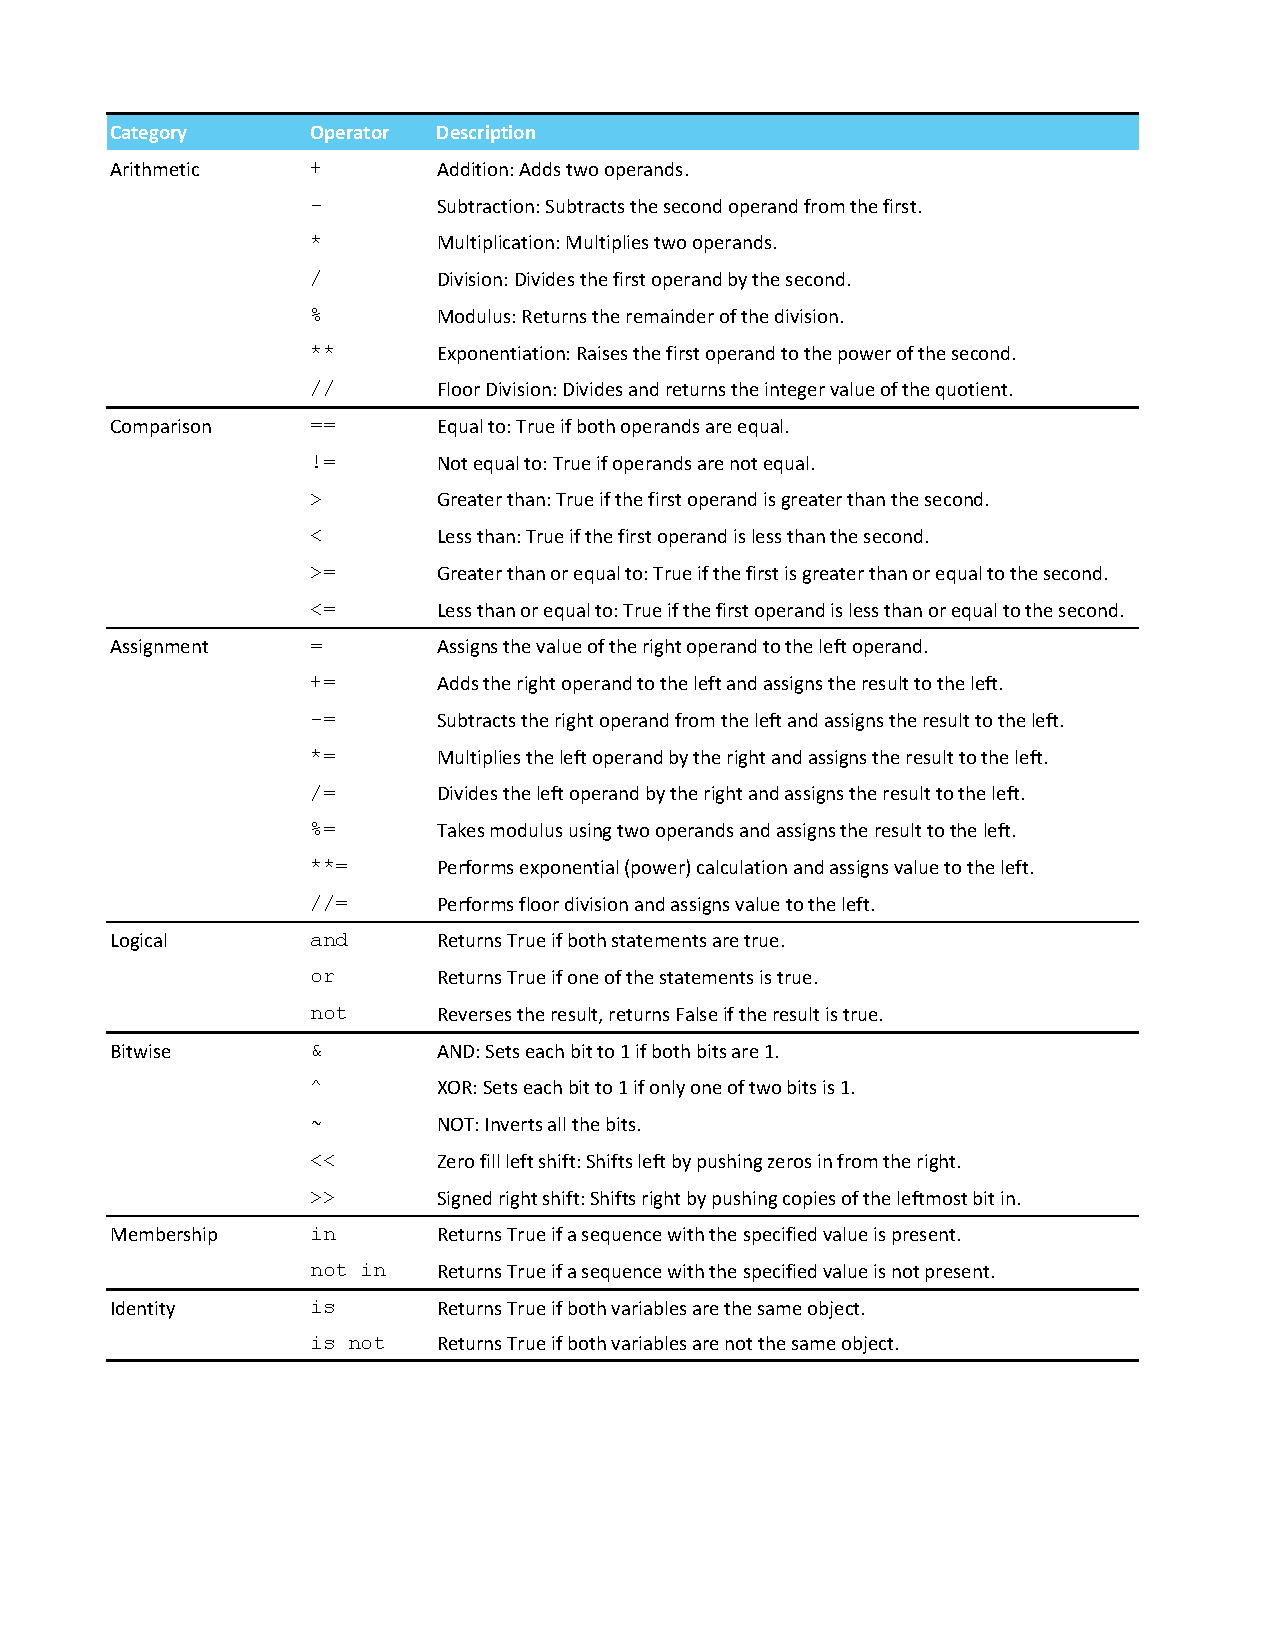
\includegraphics[width=1.0\linewidth]{Figures/Operator/Operator.pdf}
    \caption{Operators}
    \label{fig:operator}
\end{figure}